%% bare_conf.tex
%% V1.3
%% 2007/01/11
%% by Michael Shell
%% See:
%% http://www.michaelshell.org/
%% for current contact information.
%%
%% This is a skeleton file demonstrating the use of IEEEtran.cls
%% (requires IEEEtran.cls version 1.7 or later) with an IEEE conference paper.
%%
%% Support sites:
%% http://www.michaelshell.org/tex/ieeetran/
%% http://www.ctan.org/tex-archive/macros/latex/contrib/IEEEtran/
%% and
%% http://www.ieee.org/

%%*************************************************************************
%% Legal Notice:
%% This code is offered as-is without any warranty either expressed or
%% implied; without even the implied warranty of MERCHANTABILITY or
%% FITNESS FOR A PARTICULAR PURPOSE! 
%% User assumes all risk.
%% In no event shall IEEE or any contributor to this code be liable for
%% any damages or losses, including, but not limited to, incidental,
%% consequential, or any other damages, resulting from the use or misuse
%% of any information contained here.
%%
%% All comments are the opinions of their respective authors and are not
%% necessarily endorsed by the IEEE.
%%
%% This work is distributed under the LaTeX Project Public License (LPPL)
%% ( http://www.latex-project.org/ ) version 1.3, and may be freely used,
%% distributed and modified. A copy of the LPPL, version 1.3, is included
%% in the base LaTeX documentation of all distributions of LaTeX released
%% 2003/12/01 or later.
%% Retain all contribution notices and credits.
%% ** Modified files should be clearly indicated as such, including  **
%% ** renaming them and changing author support contact information. **
%%
%% File list of work: IEEEtran.cls, IEEEtran_HOWTO.pdf, bare_adv.tex,
%%                    bare_conf.tex, bare_jrnl.tex, bare_jrnl_compsoc.tex
%%*************************************************************************

% *** Authors should verify (and, if needed, correct) their LaTeX system  ***
% *** with the testflow diagnostic prior to trusting their LaTeX platform ***
% *** with production work. IEEE's font choices can trigger bugs that do  ***
% *** not appear when using other class files.                            ***
% The testflow support page is at:
% http://www.michaelshell.org/tex/testflow/



% Note that the a4paper option is mainly intended so that authors in
% countries using A4 can easily print to A4 and see how their papers will
% look in print - the typesetting of the document will not typically be
% affected with changes in paper size (but the bottom and side margins will).
% Use the testflow package mentioned above to verify correct handling of
% both paper sizes by the user's LaTeX system.
%
% Also note that the "draftcls" or "draftclsnofoot", not "draft", option
% should be used if it is desired that the figures are to be displayed in
% draft mode.
%
\documentclass[conference]{IEEEtran}
% Add the compsoc option for Computer Society conferences.
%
% If IEEEtran.cls has not been installed into the LaTeX system files,
% manually specify the path to it like:
% \documentclass[conference]{../sty/IEEEtran}





% Some very useful LaTeX packages include:
% (uncomment the ones you want to load)


% *** MISC UTILITY PACKAGES ***
%
%\usepackage{ifpdf}
% Heiko Oberdiek's ifpdf.sty is very useful if you need conditional
% compilation based on whether the output is pdf or dvi.
% usage:
% \ifpdf
%   % pdf code
% \else
%   % dvi code
% \fi
% The latest version of ifpdf.sty can be obtained from:
% http://www.ctan.org/tex-archive/macros/latex/contrib/oberdiek/
% Also, note that IEEEtran.cls V1.7 and later provides a builtin
% \ifCLASSINFOpdf conditional that works the same way.
% When switching from latex to pdflatex and vice-versa, the compiler may
% have to be run twice to clear warning/error messages.






% *** CITATION PACKAGES ***
%
\usepackage{cite}
% cite.sty was written by Donald Arseneau
% V1.6 and later of IEEEtran pre-defines the format of the cite.sty package
% \cite{} output to follow that of IEEE. Loading the cite package will
% result in citation numbers being automatically sorted and properly
% "compressed/ranged". e.g., [1], [9], [2], [7], [5], [6] without using
% cite.sty will become [1], [2], [5]--[7], [9] using cite.sty. cite.sty's
% \cite will automatically add leading space, if needed. Use cite.sty's
% noadjust option (cite.sty V3.8 and later) if you want to turn this off.
% cite.sty is already installed on most LaTeX systems. Be sure and use
% version 4.0 (2003-05-27) and later if using hyperref.sty. cite.sty does
% not currently provide for hyperlinked citations.
% The latest version can be obtained at:
% http://www.ctan.org/tex-archive/macros/latex/contrib/cite/
% The documentation is contained in the cite.sty file itself.






% *** GRAPHICS RELATED PACKAGES ***
%
\ifCLASSINFOpdf
   \usepackage[pdftex]{graphicx}
  % declare the path(s) where your graphic files are
  % \graphicspath{{../pdf/}{../jpeg/}}
  % and their extensions so you won't have to specify these with
  % every instance of \includegraphics
  % \DeclareGraphicsExtensions{.pdf,.jpeg,.png}
\else
  % or other class option (dvipsone, dvipdf, if not using dvips). graphicx
  % will default to the driver specified in the system graphics.cfg if no
  % driver is specified.
  % \usepackage[dvips]{graphicx}
  % declare the path(s) where your graphic files are
  % \graphicspath{{../eps/}}
  % and their extensions so you won't have to specify these with
  % every instance of \includegraphics
  % \DeclareGraphicsExtensions{.eps}
\fi
% graphicx was written by David Carlisle and Sebastian Rahtz. It is
% required if you want graphics, photos, etc. graphicx.sty is already
% installed on most LaTeX systems. The latest version and documentation can
% be obtained at: 
% http://www.ctan.org/tex-archive/macros/latex/required/graphics/
% Another good source of documentation is "Using Imported Graphics in
% LaTeX2e" by Keith Reckdahl which can be found as epslatex.ps or
% epslatex.pdf at: http://www.ctan.org/tex-archive/info/
%
% latex, and pdflatex in dvi mode, support graphics in encapsulated
% postscript (.eps) format. pdflatex in pdf mode supports graphics
% in .pdf, .jpeg, .png and .mps (metapost) formats. Users should ensure
% that all non-photo figures use a vector format (.eps, .pdf, .mps) and
% not a bitmapped formats (.jpeg, .png). IEEE frowns on bitmapped formats
% which can result in "jaggedy"/blurry rendering of lines and letters as
% well as large increases in file sizes.
%
% You can find documentation about the pdfTeX application at:
% http://www.tug.org/applications/pdftex





% *** MATH PACKAGES ***
%
\usepackage[cmex10]{amsmath}
% A popular package from the American Mathematical Society that provides
% many useful and powerful commands for dealing with mathematics. If using
% it, be sure to load this package with the cmex10 option to ensure that
% only type 1 fonts will utilized at all point sizes. Without this option,
% it is possible that some math symbols, particularly those within
% footnotes, will be rendered in bitmap form which will result in a
% document that can not be IEEE Xplore compliant!
%
% Also, note that the amsmath package sets \interdisplaylinepenalty to 10000
% thus preventing page breaks from occurring within multiline equations. Use:
%\interdisplaylinepenalty=2500
% after loading amsmath to restore such page breaks as IEEEtran.cls normally
% does. amsmath.sty is already installed on most LaTeX systems. The latest
% version and documentation can be obtained at:
% http://www.ctan.org/tex-archive/macros/latex/required/amslatex/math/





% *** SPECIALIZED LIST PACKAGES ***
%
%\usepackage{algorithmic}
% algorithmic.sty was written by Peter Williams and Rogerio Brito.
% This package provides an algorithmic environment fo describing algorithms.
% You can use the algorithmic environment in-text or within a figure
% environment to provide for a floating algorithm. Do NOT use the algorithm
% floating environment provided by algorithm.sty (by the same authors) or
% algorithm2e.sty (by Christophe Fiorio) as IEEE does not use dedicated
% algorithm float types and packages that provide these will not provide
% correct IEEE style captions. The latest version and documentation of
% algorithmic.sty can be obtained at:
% http://www.ctan.org/tex-archive/macros/latex/contrib/algorithms/
% There is also a support site at:
% http://algorithms.berlios.de/index.html
% Also of interest may be the (relatively newer and more customizable)
% algorithmicx.sty package by Szasz Janos:
% http://www.ctan.org/tex-archive/macros/latex/contrib/algorithmicx/




% *** ALIGNMENT PACKAGES ***
%
%\usepackage{array}
% Frank Mittelbach's and David Carlisle's array.sty patches and improves
% the standard LaTeX2e array and tabular environments to provide better
% appearance and additional user controls. As the default LaTeX2e table
% generation code is lacking to the point of almost being broken with
% respect to the quality of the end results, all users are strongly
% advised to use an enhanced (at the very least that provided by array.sty)
% set of table tools. array.sty is already installed on most systems. The
% latest version and documentation can be obtained at:
% http://www.ctan.org/tex-archive/macros/latex/required/tools/


%\usepackage{mdwmath}
%\usepackage{mdwtab}
% Also highly recommended is Mark Wooding's extremely powerful MDW tools,
% especially mdwmath.sty and mdwtab.sty which are used to format equations
% and tables, respectively. The MDWtools set is already installed on most
% LaTeX systems. The lastest version and documentation is available at:
% http://www.ctan.org/tex-archive/macros/latex/contrib/mdwtools/


% IEEEtran contains the IEEEeqnarray family of commands that can be used to
% generate multiline equations as well as matrices, tables, etc., of high
% quality.


%\usepackage{eqparbox}
% Also of notable interest is Scott Pakin's eqparbox package for creating
% (automatically sized) equal width boxes - aka "natural width parboxes".
% Available at:
% http://www.ctan.org/tex-archive/macros/latex/contrib/eqparbox/





% *** SUBFIGURE PACKAGES ***
%\usepackage[tight,footnotesize]{subfigure}
% subfigure.sty was written by Steven Douglas Cochran. This package makes it
% easy to put subfigures in your figures. e.g., "Figure 1a and 1b". For IEEE
% work, it is a good idea to load it with the tight package option to reduce
% the amount of white space around the subfigures. subfigure.sty is already
% installed on most LaTeX systems. The latest version and documentation can
% be obtained at:
% http://www.ctan.org/tex-archive/obsolete/macros/latex/contrib/subfigure/
% subfigure.sty has been superceeded by subfig.sty.



%\usepackage[caption=false]{caption}
%\usepackage[font=footnotesize]{subfig}
% subfig.sty, also written by Steven Douglas Cochran, is the modern
% replacement for subfigure.sty. However, subfig.sty requires and
% automatically loads Axel Sommerfeldt's caption.sty which will override
% IEEEtran.cls handling of captions and this will result in nonIEEE style
% figure/table captions. To prevent this problem, be sure and preload
% caption.sty with its "caption=false" package option. This is will preserve
% IEEEtran.cls handing of captions. Version 1.3 (2005/06/28) and later 
% (recommended due to many improvements over 1.2) of subfig.sty supports
% the caption=false option directly:
%\usepackage[caption=false,font=footnotesize]{subfig}
%
% The latest version and documentation can be obtained at:
% http://www.ctan.org/tex-archive/macros/latex/contrib/subfig/
% The latest version and documentation of caption.sty can be obtained at:
% http://www.ctan.org/tex-archive/macros/latex/contrib/caption/




% *** FLOAT PACKAGES ***
%
%\usepackage{fixltx2e}
% fixltx2e, the successor to the earlier fix2col.sty, was written by
% Frank Mittelbach and David Carlisle. This package corrects a few problems
% in the LaTeX2e kernel, the most notable of which is that in current
% LaTeX2e releases, the ordering of single and double column floats is not
% guaranteed to be preserved. Thus, an unpatched LaTeX2e can allow a
% single column figure to be placed prior to an earlier double column
% figure. The latest version and documentation can be found at:
% http://www.ctan.org/tex-archive/macros/latex/base/



%\usepackage{stfloats}
% stfloats.sty was written by Sigitas Tolusis. This package gives LaTeX2e
% the ability to do double column floats at the bottom of the page as well
% as the top. (e.g., "\begin{figure*}[!b]" is not normally possible in
% LaTeX2e). It also provides a command:
%\fnbelowfloat
% to enable the placement of footnotes below bottom floats (the standard
% LaTeX2e kernel puts them above bottom floats). This is an invasive package
% which rewrites many portions of the LaTeX2e float routines. It may not work
% with other packages that modify the LaTeX2e float routines. The latest
% version and documentation can be obtained at:
% http://www.ctan.org/tex-archive/macros/latex/contrib/sttools/
% Documentation is contained in the stfloats.sty comments as well as in the
% presfull.pdf file. Do not use the stfloats baselinefloat ability as IEEE
% does not allow \baselineskip to stretch. Authors submitting work to the
% IEEE should note that IEEE rarely uses double column equations and
% that authors should try to avoid such use. Do not be tempted to use the
% cuted.sty or midfloat.sty packages (also by Sigitas Tolusis) as IEEE does
% not format its papers in such ways.





% *** PDF, URL AND HYPERLINK PACKAGES ***
%
%\usepackage{url}
% url.sty was written by Donald Arseneau. It provides better support for
% handling and breaking URLs. url.sty is already installed on most LaTeX
% systems. The latest version can be obtained at:
% http://www.ctan.org/tex-archive/macros/latex/contrib/misc/
% Read the url.sty source comments for usage information. Basically,
% \url{my_url_here}.





% *** Do not adjust lengths that control margins, column widths, etc. ***
% *** Do not use packages that alter fonts (such as pslatex).         ***
% There should be no need to do such things with IEEEtran.cls V1.6 and later.
% (Unless specifically asked to do so by the journal or conference you plan
% to submit to, of course. )


% correct bad hyphenation here
\hyphenation{op-tical net-works semi-conduc-tor}


\begin{document}
%
% paper title
% can use linebreaks \\ within to get better formatting as desired
\title{Mathematical modelling of artificial heart valve performance}


% author names and affiliations
% use a multiple column layout for up to three different
% affiliations
\author{
    \IEEEauthorblockN{Dmitriy Dolgov}
    \IEEEauthorblockA{Kemerovo State University\\
    Email: 9erthalion6@gmail.com}
    \and
    \IEEEauthorblockN{Yury Zakharov}
    \IEEEauthorblockA{Kemerovo State University\\
    Email: zaxarov@rambler.ru}
}

% conference papers do not typically use \thanks and this command
% is locked out in conference mode. If really needed, such as for
% the acknowledgment of grants, issue a \IEEEoverridecommandlockouts
% after \documentclass

% for over three affiliations, or if they all won't fit within the width
% of the page, use this alternative format:
% 
%\author{\IEEEauthorblockN{Michael Shell\IEEEauthorrefmark{1},
%Homer Simpson\IEEEauthorrefmark{2},
%James Kirk\IEEEauthorrefmark{3}, 
%Montgomery Scott\IEEEauthorrefmark{3} and
%Eldon Tyrell\IEEEauthorrefmark{4}}
%\IEEEauthorblockA{\IEEEauthorrefmark{1}School of Electrical and Computer Engineering\\
%Georgia Institute of Technology,
%Atlanta, Georgia 30332--0250\\ Email: see http://www.michaelshell.org/contact.html}
%\IEEEauthorblockA{\IEEEauthorrefmark{2}Twentieth Century Fox, Springfield, USA\\
%Email: homer@thesimpsons.com}
%\IEEEauthorblockA{\IEEEauthorrefmark{3}Starfleet Academy, San Francisco, California 96678-2391\\
%Telephone: (800) 555--1212, Fax: (888) 555--1212}
%\IEEEauthorblockA{\IEEEauthorrefmark{4}Tyrell Inc., 123 Replicant Street, Los Angeles, California 90210--4321}}




% use for special paper notices
%\IEEEspecialpapernotice{(Invited Paper)}




% make the title area
\maketitle


\begin{abstract}
%\boldmath
The paper is dedicated to the mathematical model describing dynamics of blood circulation in an artificial heart valve and its computational solution algorithm. The model estimated values of tricuspid valve performance are presented.
\end{abstract}
% IEEEtran.cls defaults to using nonbold math in the Abstract.
% This preserves the distinction between vectors and scalars. However,
% if the conference you are submitting to favors bold math in the abstract,
% then you can use LaTeX's standard command \boldmath at the very start
% of the abstract to achieve this. Many IEEE journals/conferences frown on
% math in the abstract anyway.

% no keywords




% For peer review papers, you can put extra information on the cover
% page as needed:
% \ifCLASSOPTIONpeerreview
% \begin{center} \bfseries EDICS Category: 3-BBND \end{center}
% \fi
%
% For peerreview papers, this IEEEtran command inserts a page break and
% creates the second title. It will be ignored for other modes.
\IEEEpeerreviewmaketitle



\section{Introduction}
% no \IEEEPARstart
Artificial heart valves are proved to be an effective mode of many 
cardiovascular diseases treatment. Annually approximately 250 000 surgeries 
are performed in the world to restore or replace damaged heart valves and the 
quantity is expected to increase \cite{yacoub}. However, artificial heart valves are 
considered to be complex medical devices used in cardio surgery because of 
their design features. A valve is required to minimize turbulence, help to avoid 
stagnation zones, flow separation, etc.  Mathematical modelling of artificial 
heart valves performance enables to get thorough understanding of its internal 
processes in order to improve its design due to the parameters under 
consideration. Sometimes experimental methods can’t cope with this task.
There are many researches dedicated to modelling and numerical calculation of 
a leaflet valve performance problem. One of the popular approaches analyzes 
mechanical characteristics of the valve that is effected by the pressure, its 
tensions and deformations \cite{bokeria, kim}. Such kind of researches considers only a valve 
itself while ignoring flow which influences this valve. It is obviously a 
disadvantage. In order to build a major model of a valve it’s necessary to take 
into consideration the “valve-flow” interaction. Its numerical implementation 
may cause great difficulties, since a valve leaflets are very thin and flexible and 
flow inside the valve has a complex structure. Two main problem solution 
approaches are usually defined. First approach is related to the finite element 
methods \cite{zhang, black}. They enable to take into consideration complex geometry of 
a valve and a vessel but the necessity of taking into account the interaction 
between fluid and flexible walls requires constant rebuilding of the 
computational grid to meet the changing geometry of the object under 
investigation. It appears to be time and computational resources consuming.
The second approach, which is related to the immersed boundary method, is 
under discussion in this paper \cite{pescin_2002, griffith_2011, ma_x_2013, jian}. It can be used to solve the problems with 
complex geometry, and it doesn't require grid modification.
We propose to describe the blood flow in the flexible large blood vessels and the 
artificial heart valve as a three dimensional nonstationary flow of viscous 
incompressible fluid with variable viscosity and density (see \cite{gummel, geidarov, milosevic, dolgov}, Fig. \ref{fig:heart_scheme}).
Thus, the goal of this work is to develop a mathematical model and a solution 
method of the problem of artificial heart leaflet dynamics inside a blood vessel 
taking into account the inhomogeneous blood structure.

\section{Problem formulation}
Vessel walls and valve leaflets consist of a large number of thin collagen fibers; 
they can change their form depending on the blood flow. Valve leaflets are very 
thin, their bases are attached to a hard fibrous ring. Blood consists of plasma and 
formed elements, which are approximately 45\% of the entire volume.

\begin{figure}[!t]
\centering
\includegraphics[width=2.0in]{images/heart_scheme.png}
\caption{Aortic valve and its location inside heart}
\label{fig:heart_scheme}
\end{figure}

Since blood circulates through vessels under the pressure created by cardiac 
beats then the problem of the blood flow can be described by Navier-Stokes 
nonstationary system of differential equations \cite{gummel}:

\begin{figure}[!t]
\centering
\includegraphics[width=2.5in]{images/area_3d.png}
\caption{Computational domain boundaries}
\label{fig:area_3d}
\end{figure}

\begin{gather}
    \label{eq:navier_stokes:motion}
    \frac{\partial \vec{u}}{\partial t} + (\vec{u} \cdot \nabla) \vec{u} = - \frac{1}{\rho} \nabla p + \nabla \sigma + \vec{f}\\
    \label{eq:navier_stokes:continuity}
    \frac{\partial \rho}{\partial t} + \nabla \cdot (\rho \vec{u}) = 0 
\end{gather}

with the initial and boundary conditions:

\begin{gather}
    \label{eq:navier_stokes:velocity_conditions}
    \vec{u}(\bar{x}, 0) = \vec{u}_0 \qquad \vec{u}|_{\Gamma_1, \Gamma_4} = \vec{u}_b \qquad u_{\Gamma_2, \Gamma3} = 0\\
    \label{eq:navier_stokes:pressure_conditions}
    p_{\Gamma_2} = p_{in} \qquad p_{\Gamma_3} = p_{out}
\end{gather}

where $\bar{x}=(x,y,z) \in \Omega$, $\vec{u}=(u,v,w)$ - velocity vector, $u, v, w$ - $x$-, $y$-, $z$-components of velocity vector,
$\vec{u}_b$ - velocity of the vessel walls and valve leaflets motion under deformation,
$\rho=\rho(\bar{x}, t)$ - density, $p=p(\bar{x}, t)$ - pressure, $\sigma = \mu (\nabla \vec{u} + (\nabla \vec{u})^T)$ - viscous stress tensor,
$\mu = \mu(\bar{x}, t)$ - fluid viscosity, $\vec{f} = \vec{f}(\bar{x}, t)$ - body forces vector, which is further used to determine form of the vessel and valve leaflets.
Domain $\Omega$ is a vessel with boundary $\Gamma = \Gamma_1 \cup \Gamma_2 \cup \Gamma_3 \cup \Gamma_4$, where $\Gamma_1$ - blood vessel wall,
$\Gamma_2$ and $\Gamma_3$ - inflow and outflow domains, $\Gamma_4$ - valve leaflets (see Fig. \ref{fig:area_3d}).

Density $\rho$ and viscosity $\mu$ are defined by following relations \cite{gummel}:
\begin{gather}
    \label{eq:viscosity}
    \mu = c (\mu_2 - \mu_1) + \mu_1\\
    \label{eq:density}
    \rho = c (\rho_2 - \rho_1) + \rho_1
\end{gather}

where $\rho_1$, $\mu_1$ - fluid density and viscosity (plasma), $\rho_2$, $\mu_2$ - admixture density and viscosity (formed elements), $c$ - admixture concentration.
Admixture concentration $c=c(\bar{x}, t)$, $c \in [0, 1]$ is determined as a solution of equation:
\begin{gather}
    \label{eq:convection}
    \frac{\partial c}{\partial t} + \vec{u} \cdot \nabla c = 0
\end{gather}

with initial conditions:
\begin{gather}
    \label{eq:convection:conditions}
    c(\bar{x}, 0) = c_0(\bar{x}), \bar{x} \in \Omega
\end{gather}

and boundary conditions at the inflow boundary:
\begin{gather}
    \label{eq:convection:conditions}
    c(\bar{x}, t)|_{\Gamma_2} = c_s(\bar{x}, t)
\end{gather}

where $c_0, c_s$ are specified functions. 
One of the issues determined for this kind of problem computational solutions is the lack of one component of velocity vector in the inflow-outflow areas.
It can be solved by using the original equations (\ref{eq:navier_stokes:motion}) - (\ref{eq:navier_stokes:pressure_conditions}) at the boundaries
$\Gamma_2$, $\Gamma_3$ to determine the missing components of the velocity vector (see details \cite{gummel, geidarov, milosevic}).

Motion of the vessel walls and valve leaflets is defined by the forces, which return them to the original position. Valve leaflets can be deformated much more,
than vessel walls. To describe the forces, arising due to the valve deformation, the following formula is used:

\begin{gather}
    \label{eq:boundary_force}
    F = \frac{\partial}{\partial s} (T \tau) + \frac{\partial^2}{\partial s^2} (E \cdot I \frac{\partial^2}{\partial s^2} X)
\end{gather}

where $\bar{q} = (q, r, s) \in \Gamma_4$, $X(\bar{q})$ - function for describing the valve leaflets surface at the moment $t$, the coordinates $q, r, s$ are chosen 
so that the surface $X$ is presented by the large amount of parametric lines $s \rightarrow X(q^0, r^0, s)$, $T$ - tension,
that arises due to the stretching along $s$, $E$ - Young's modulus, $I$ - cross-sectional moment of inertia (see \cite{griffith_2011}).

Researches \cite{pescin_2002, griffith_2011} show, that in order to the interaction between vessel walls, valve leaflets and the fluid flow it is necessary
to compute the field of external body forces $f$ in the Navier-Stokes equation, based on the force $F$, and determine the current form $X(\bar{q}, t)$ 
of the vessel and the valve, based on the fluid field of velocities $\vec{u}(\bar{x}, t)$. The following equations are used for this purpose:
\begin{gather}
    \label{eq:interaction:velocity}
    \frac{\partial X}{\partial t}(\bar{q}, t) = \int_{\Omega} \vec{u}(\bar{x}, t) \cdot \delta (x - X(\bar{q}, t))\; dx\; dy\; dz\\
    \label{eq:interaction:force}
    \vec{f}(\bar{x}, t) = \int_{\Gamma} \vec{F}(\bar{q}, t) \cdot \delta (x - X(\bar{q}, t))\; dq\; dr\; ds
\end{gather}

where $\bar{q} = (q, r, s) \in \Gamma$ - point at the vessel wall or valve leaflet, $X = X(\bar{q}, t)$ - function for describing the vessel
and valve surfaces at the moment $t$, $F = F(\bar{q}, t)$ - the force of deformation resistance at given point,
$\vec{u}(\bar{x}, t)$ - fluid flow velocity vector, $\vec{f}(\bar{x}, t)$ - body forces vector, $\delta$ - Dirac delta function.

Thus the model describing the motion of the viscous inhomogeneous incompressible fluid inside vessel with valve is built. This model enables to determine
the fluid state and the surface form $\Gamma_1 \cup \Gamma_4$ independently of each other. The valve leaflets influence on the fluid is described by 
correlation (\ref{eq:interaction:force}) between the vector of body forces $\vec{f}(\bar{x}, t)$ from (\ref{eq:navier_stokes:motion}) 
and the force of deformation resistance $F = F(\bar{q}, t)$ from (\ref{eq:boundary_force}).

\section{Solution method}
As it was mentioned before, immersed boundary method is used in the paper \cite{pescin_2002}.

According to this method, we determine the fluid flow in the parallelepiped $\tilde{\Omega}$, which contains $\Omega$.
$\tilde{\Omega}$ has no-slip boundary conditions.
To compute of the fluid flow we use rectangular uniform staggered grid $\tilde{\Omega_h}$ with grid spacing $h_x$, $h_y$, $h_z$ and 
staggered arrangement of cells, where the pressure, velocity divergence and concentration are computed at the center of cell, the velocity vector components
and vector of external forces are computed at the boundaries of cell. To determine the deformation of the surface
$\Gamma_1 \cup \Gamma_4$ we introduce additional area $\tilde{\Gamma}$ with Lagrangian coordinate system, which is related to the vessel
walls and valve leaflets. In the $\tilde{\Gamma}$ we construct a new grid $\tilde{\Gamma_h}$, with cells corresponding to the points at the $\Gamma_1 \cup \Gamma_4$.
Solution algorithm consists of several steps:
at the grid $\tilde{\Gamma_h}$ the problem (\ref{eq:navier_stokes:motion})-(\ref{eq:navier_stokes:pressure_conditions}) is solved; then the convection equation 
(\ref{eq:convection}) is solved, i.e. the concentration of admixture is determined in the solution domain and the density and viscosity are recalculated.
Then formulas (\ref{eq:boundary_force}) and (\ref{eq:interaction:velocity}), (\ref{eq:interaction:force}) are used to
determine the position of leaflets and the vessel form.

Differential equation (\ref{eq:navier_stokes:motion}), (\ref{eq:convection:conditions}) is solved by the finite difference method.
To solve (\ref{eq:navier_stokes:motion}), (\ref{eq:navier_stokes:pressure_conditions}) splitting schemes due to physical factors are used \cite{belotserkovsky}:
\begin{gather}
    \label{eq:splitting:intermediate_velocity}
    \frac{u^* - u^n}{\triangle t} = - (u^n \cdot \nabla) u^* - \frac{1}{\rho} \nabla \sigma + f^n\\
    \label{eq:splitting:poisson}
    \rho \triangle p^{n+1} - \nabla \rho \cdot p^{n+1} = \frac{\rho^2 \nabla u^*}{\triangle t}\\
    \label{eq:splitting:velocity}
    \frac{u^{n+1} - u^*}{\triangle t} = - \frac{1}{\rho} \triangle p^{n+1}
\end{gather}

Numerical implementation of this scheme consists of three stages. At the beginning the intermediate field $u^*$  is computed using the known values of velocity
from the previous time step. Thus equation (\ref{eq:splitting:intermediate_velocity}) is solved by the method of stabilizing corrections \cite{yanenko}.
Then a new pressure field is determined via the computational solution of (\ref{eq:splitting:poisson}) using biconjugate gradient method.
At the last stage a final velocity vector field is calculated according to the formula (\ref{eq:splitting:velocity}).

As soon as fluid flow parameters are determined it is necessary to calculate new values of density and velocity. To do that a new time step for the convection
equation (\ref{eq:convection}) must be done using the obtained values of velocity components, and the density and viscosity are recalculated
by the formulas (\ref{eq:viscosity}), (\ref{eq:density}).

Next it is necessary to determine the deformation of vessel walls and valve leaflets being influenced by of fluid flow, and also the distribution of body forces $f$
in the fluid motion equation based on this deformation. It is possible to calculate the deformation of vessel walls and valve leaflets under this particular fluid pressure
and the resistance forces by using the equations (\ref{eq:interaction:velocity}) - (\ref{eq:interaction:force}), which are numerically integrated by
using any of quadrature formulas, and equation (\ref{eq:boundary_force}). Afterwards, the body forces $f$
are recalculated, and it is possible to move to the next time step.

\section{Results}
Some results of methodical calculations for the cases with constant and variable 
density and viscosity are aimed to demonstrate the described method validation 
and the possibility to get the patterns of leaflet deformation and admixture 
distribution inside them. All calculations were performed in accordance with 
dimensionless variables. A circular cylinder with length $l = 1$, radius $r = 0.11$
and wall stiffness $k = 1 \cdot 10^3$ was used as a vessel with a valve.
Valve leaflets are specified to have stretching resistance coefficient
$k_b = 5 \cdot 10^3$ and bending resistance coefficient $k_b = 5 \cdot 10^3$.
Pressure differential $p_{in} - p_{out}$ changes periodically from 0 to 6.
The domain $\tilde{\Omega}$ has parameters $1.0 \times 0.5 \times 0.5$,
spatial steps $h_x = h_y = h_k = 0.01$, time step $\triangle t = 0.01$.

Fig. \ref{fig:valve} show tricuspid valve dynamics effected by the pressure of fluid with constant density and viscosity $\rho_1 = \rho_2 = 1$, $\mu_1 = \mu_2 = 1 \cdot 10^{-2}$ and tracks of some particles.


\begin{figure}[!t]
\centering
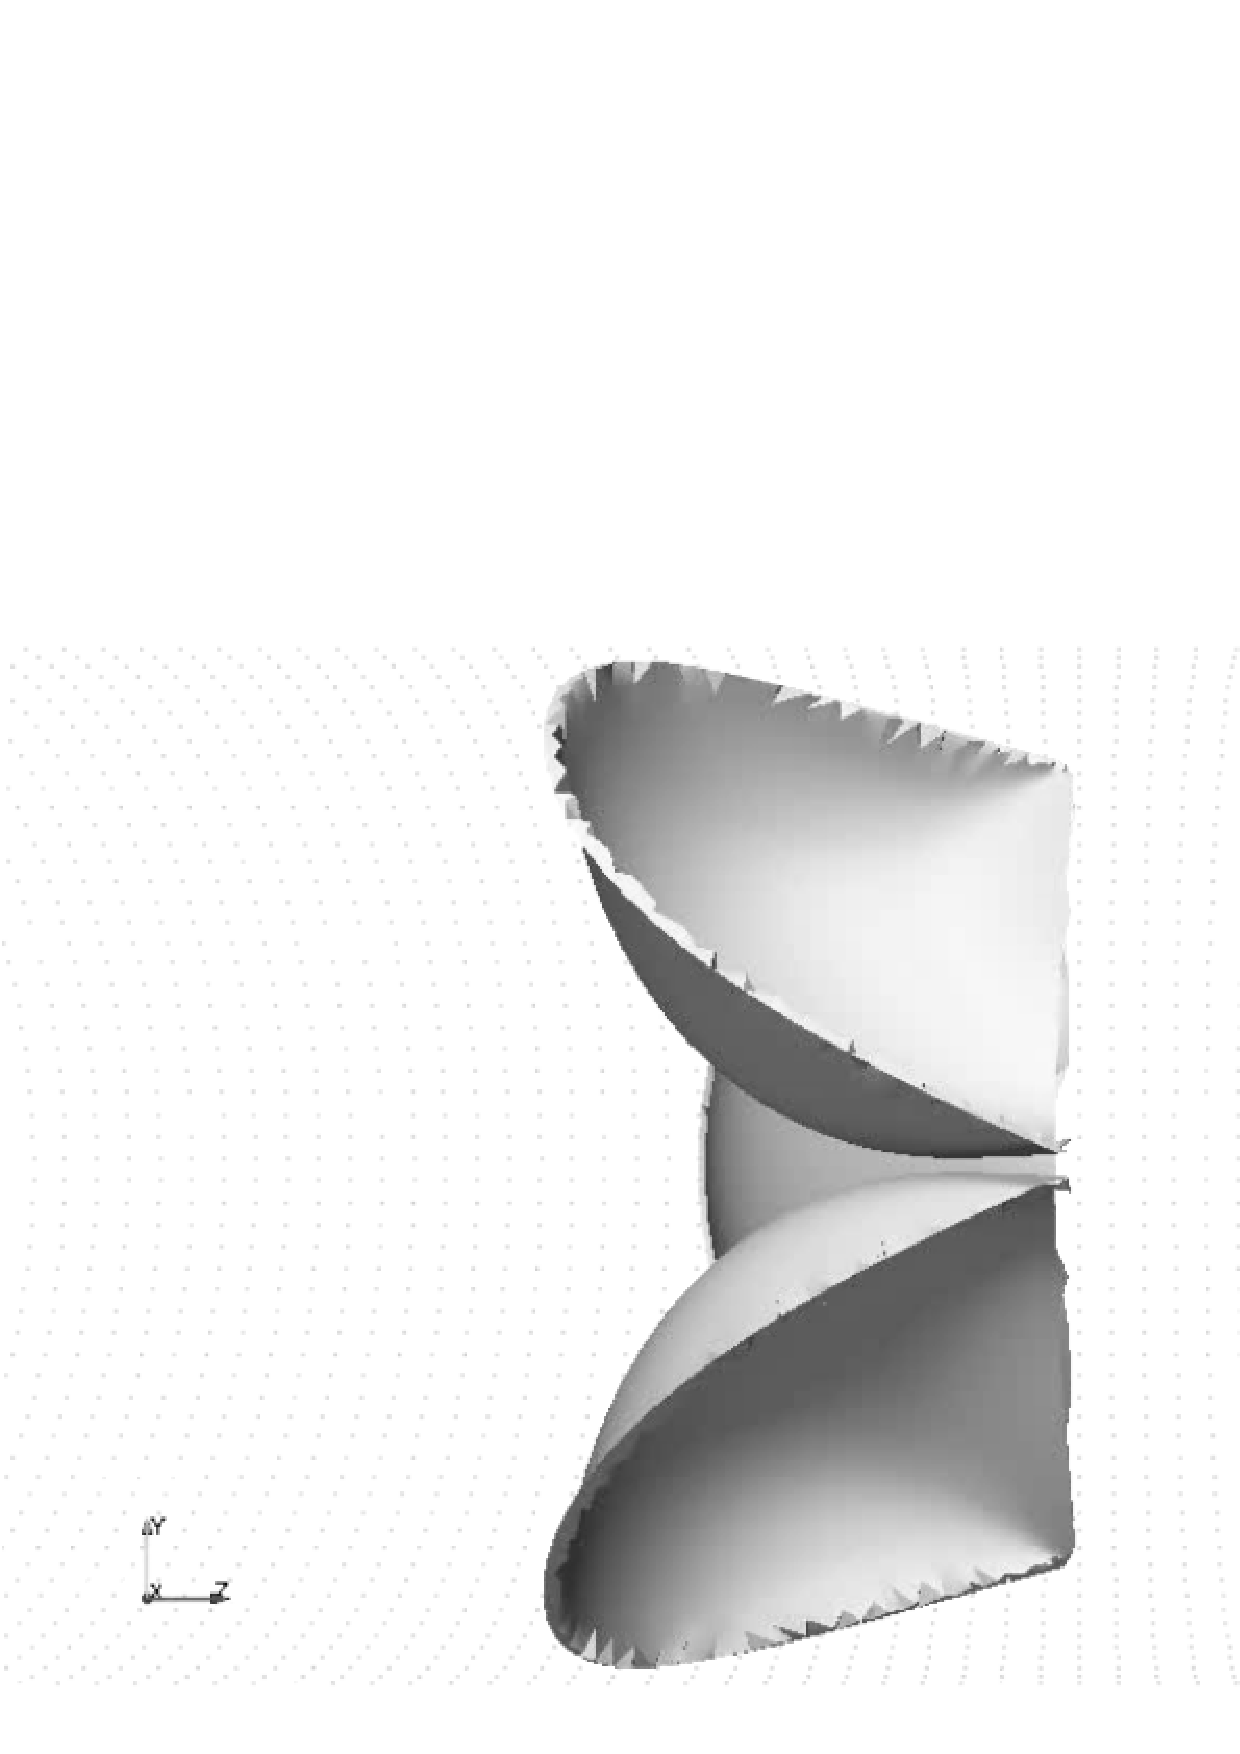
\includegraphics[width=2.5in]{images/valve_delaunay_with_markers_grayscale1.png}

$a$

\includegraphics[width=2.5in]{images/valve_delaunay_with_markers_grayscale2.png}

$b$

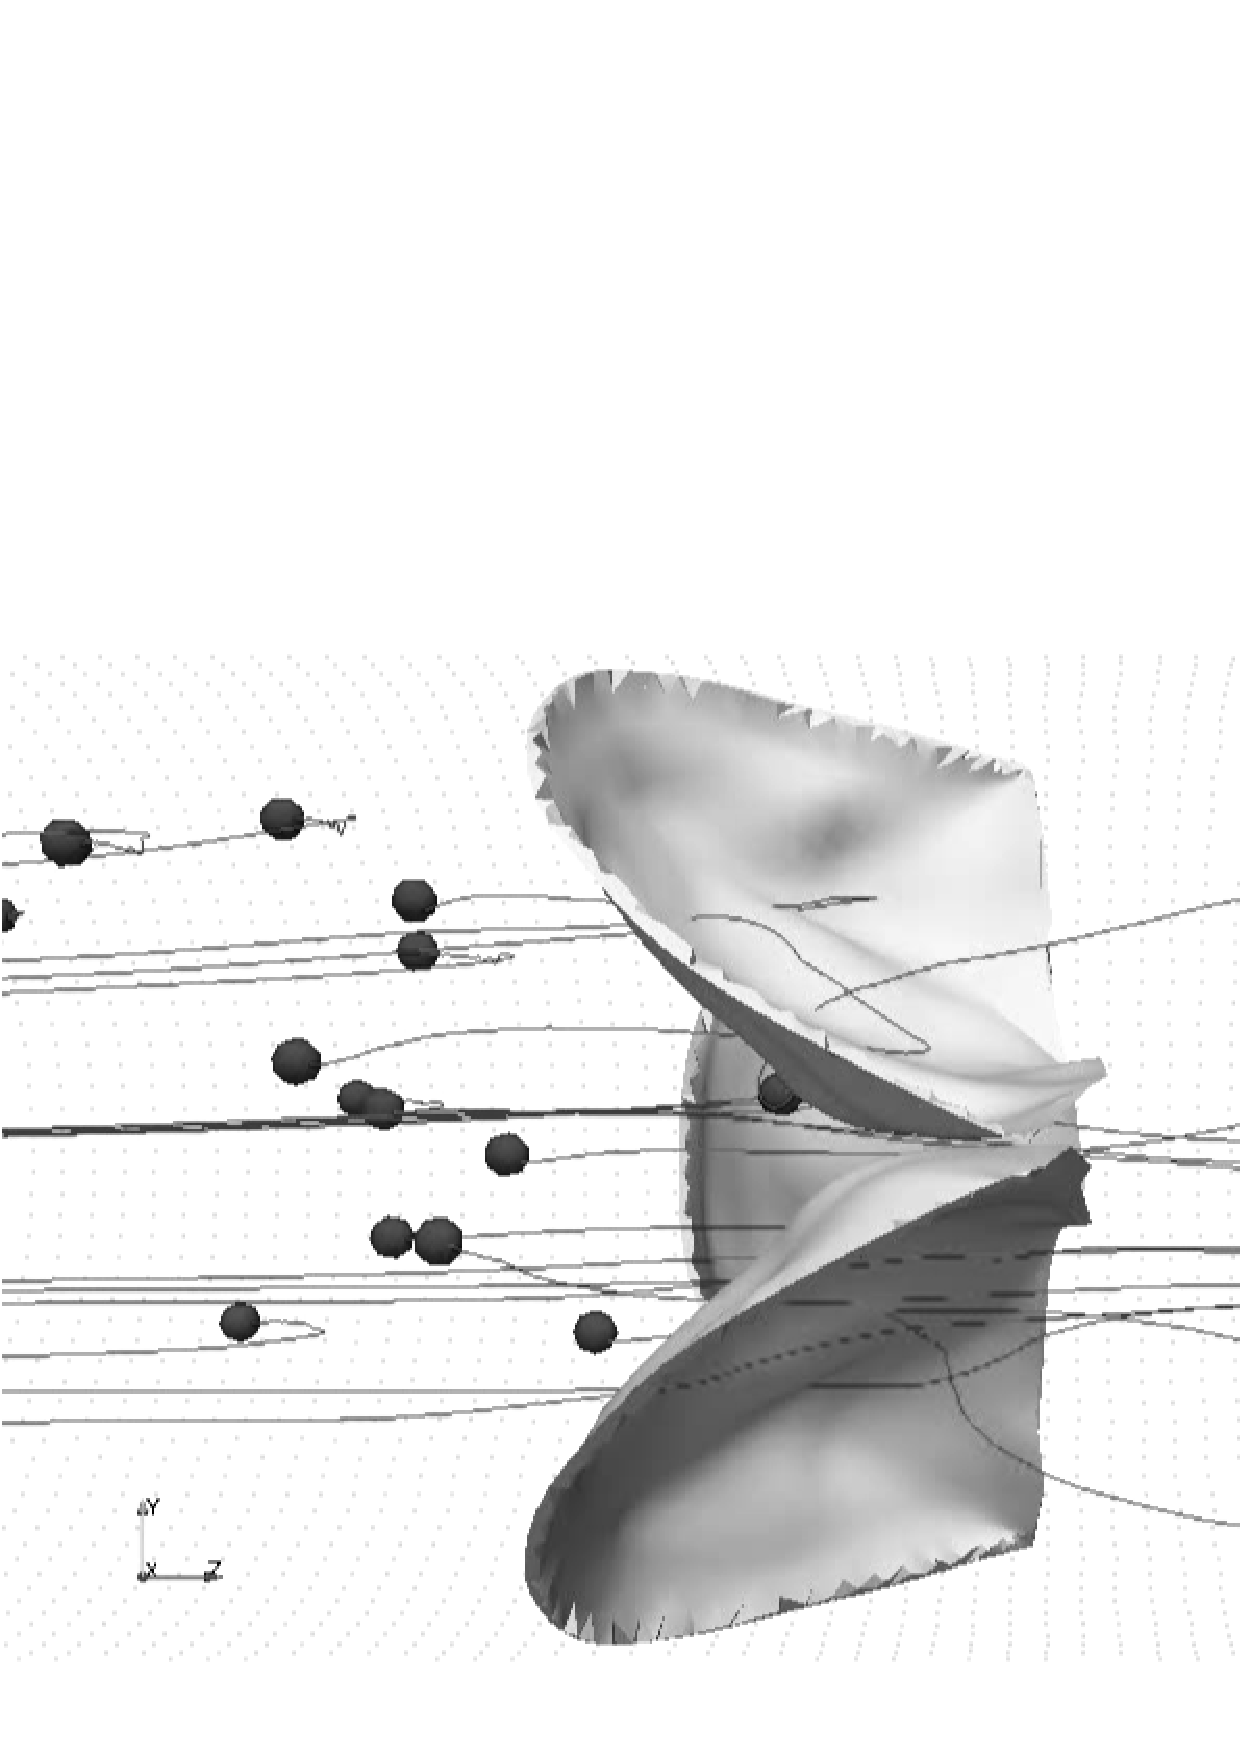
\includegraphics[width=2.5in]{images/valve_delaunay_with_markers_grayscale3.png}

$c$

\caption{Dynamics of the valve leaflets and tracks of some particles. Flow direction  is indicated by the arrow.
Side view (I, with tracks), front view (II);
a) $t=0$, b) $t=0.7$, c) $t=1.5$}
\label{fig:valve}
\end{figure}

As can be seen in the Fig. \ref{fig:valve}, the valve opens when pressure differential is increased,
and then reverts to the original state when pressure is balanced.

Fig. \ref{fig:valve_in_mixture} shows the motion dynamics of the tricuspid valve under the pressure of fluid with variable viscosity and
density $\rho_1 = \rho_2 = 1$, $\mu_1 = \mu_2 = 1 \cdot 10^{-2}$. Constant admixture flow with concentration $c_s = 0.45$ is considered at $\Gamma_2$.

\begin{figure}[!t]
\centering
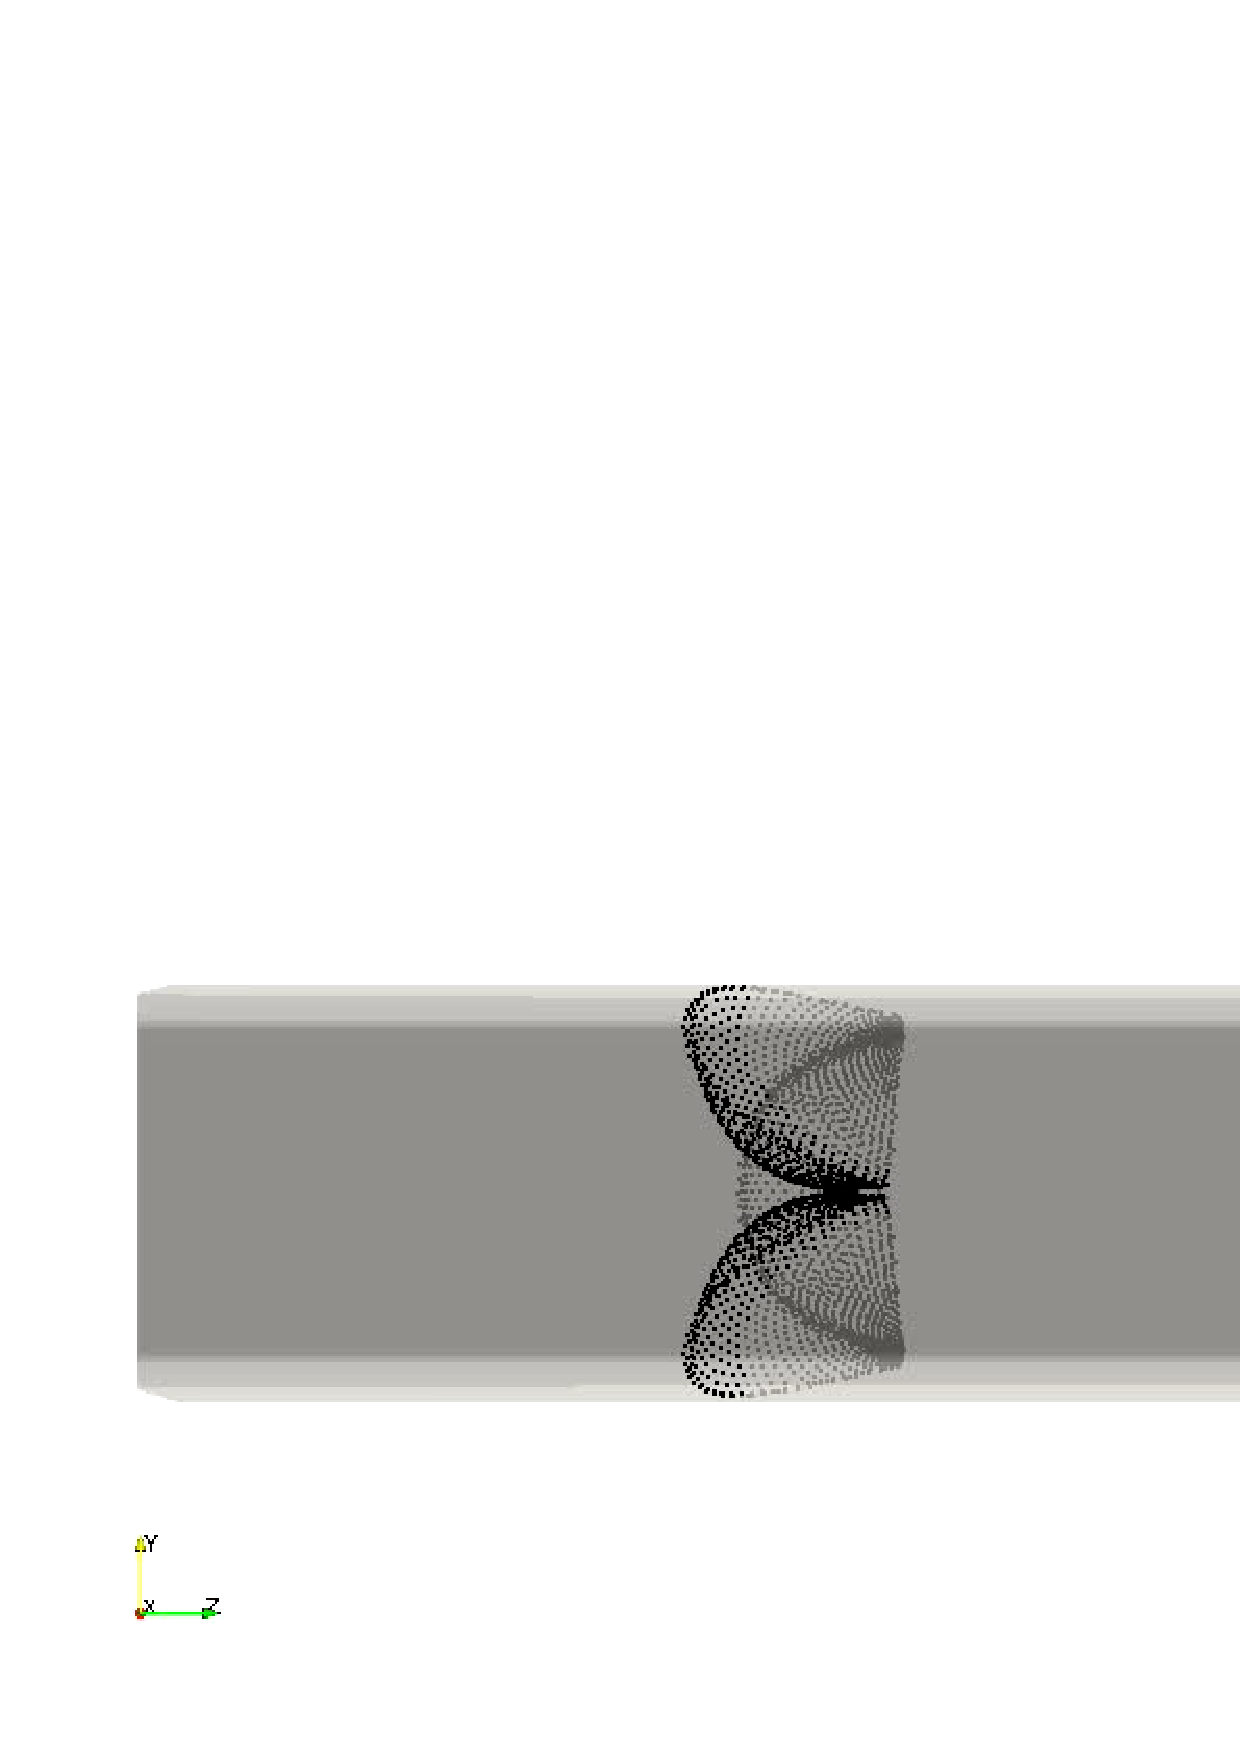
\includegraphics[width=2.5in]{images/valve_in_mixture_grayscale_new1.png}

$a$

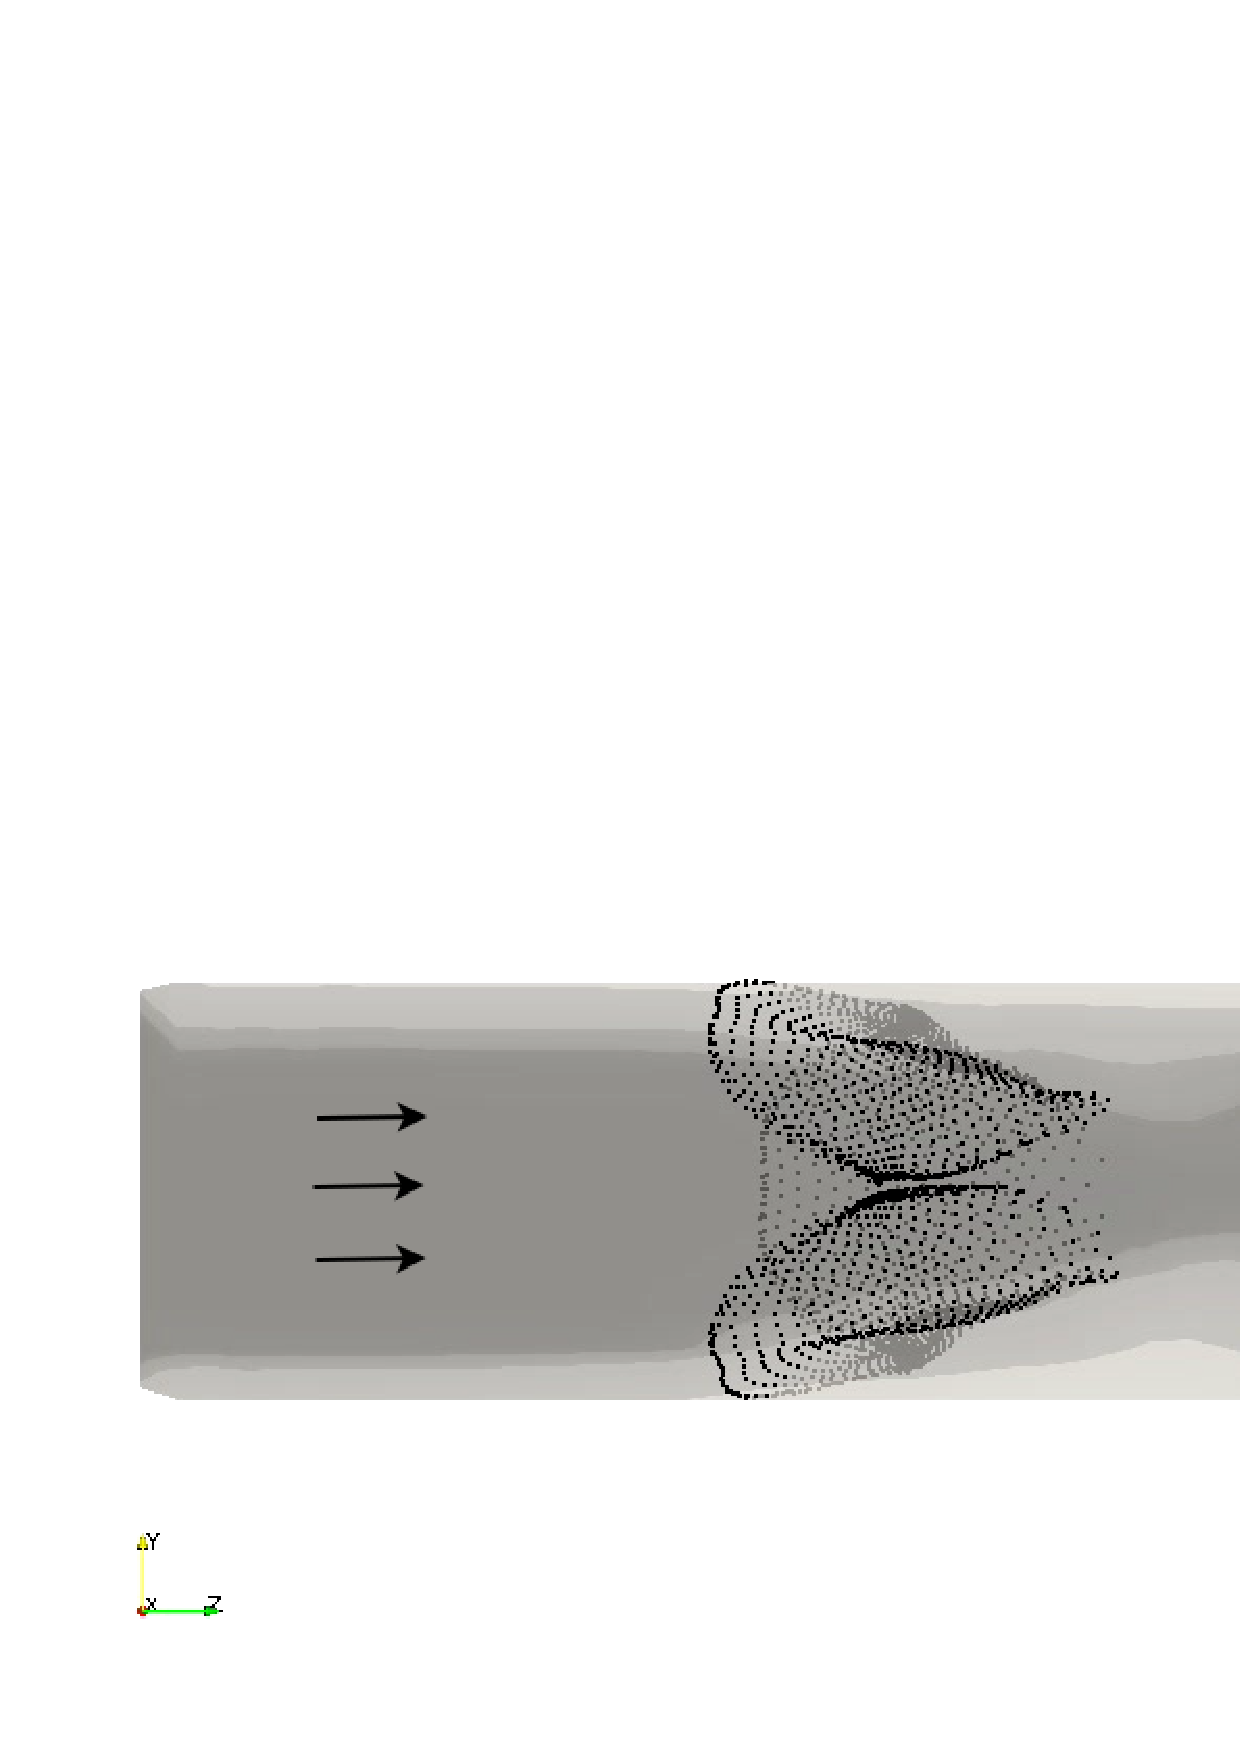
\includegraphics[width=2.5in]{images/valve_in_mixture_grayscale_new2.png}

$b$

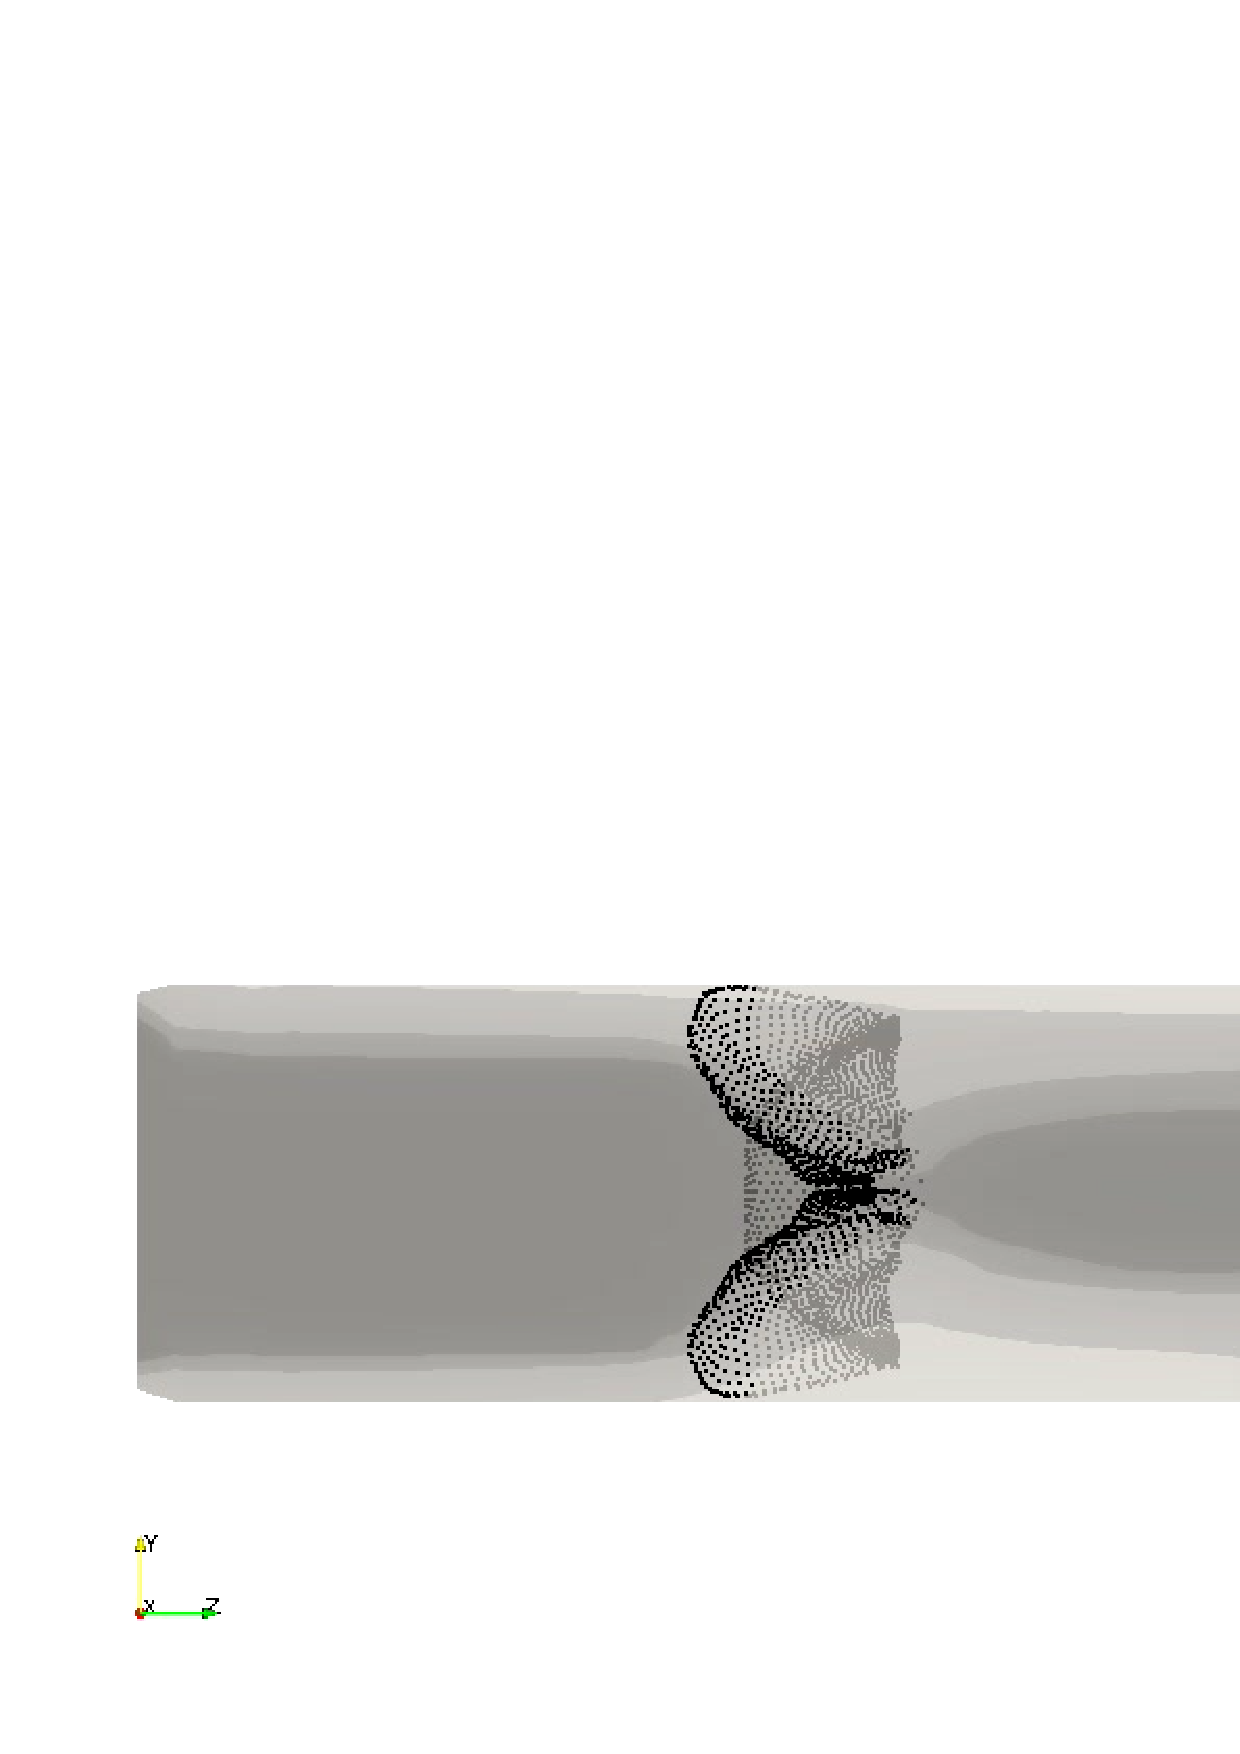
\includegraphics[width=2.5in]{images/valve_in_mixture_grayscale_new3.png}

$c$

\caption{Valve leaflets motion in a vessel with variable viscosity and density. Flow direction  is indicated by the
arrows. A constant admixture inflow $c_s|_{\Gamma_2} = 0.45$ is defined at the entrance, admixture concentration at the initial time $c_0 = 0.45$;
a) $t=0$, b) $t=0.7$, c) $t=1.5$}
\label{fig:valve_in_mixture}
\end{figure}

As can be seen in the Fig. \ref{fig:valve_in_mixture}, the initial uniform admixture distribution is interrupted by the valve leaflets motion. Eventually oscillatory mode of
admixture motion can be recognized that corresponds to valve operating cycle. 
Moreover, the Fig. \ref{fig:valve_in_mixture} shows that admixture distribution over a cross section being parallel to axis $Oy$
is not symmetric because the valve leaflets are not symmetric about the axis $Oy$ as well.

Fig. \ref{fig:flow_rate} shows diagrams of fluid flow regarding 3 operation cycles of the valve ( 
highlighted by the dotted graph) and data from the research \cite{griffith} (highlighted by 
the continuous line).  Though nondimensional values are taken into 
consideration in the paper. the diagrams show commonality. Each cycle contains 
sharp shift at the beginning, then soft attenuation with line bend and 
oscillation as soon as the valve closes. The first cycle has flows difference 
because \cite{griffith} considers the valve to be tense, so it opens less in that case.

\begin{figure}[!t]
\centering
\includegraphics[width=2.5in]{images/flow_rate_comparison_with_legend_grayscale.png}
\caption{Diagrams of fluid flow which take into consideration the parameters of Fig. \ref{fig:valve_in_mixture} (highlighted by the dotted
    graph)  and the results obtained in \cite{griffith} (highlighted by the continuous line)}
\label{fig:flow_rate}
\end{figure}

\section{Conclusion}

The constructed model of blood flow with variable viscosity and density allows 
to get the patterns of leaflet deformation and admixture distribution effected by 
inhomogeneous fluid flow.

% An example of a floating figure using the graphicx package.
% Note that \label must occur AFTER (or within) \caption.
% For figures, \caption should occur after the \includegraphics.
% Note that IEEEtran v1.7 and later has special internal code that
% is designed to preserve the operation of \label within \caption
% even when the captionsoff option is in effect. However, because
% of issues like this, it may be the safest practice to put all your
% \label just after \caption rather than within \caption{}.
%
% Reminder: the "draftcls" or "draftclsnofoot", not "draft", class
% option should be used if it is desired that the figures are to be
% displayed while in draft mode.
%
%\begin{figure}[!t]
%\centering
%\includegraphics[width=2.5in]{myfigure}
% where an .eps filename suffix will be assumed under latex, 
% and a .pdf suffix will be assumed for pdflatex; or what has been declared
% via \DeclareGraphicsExtensions.
%\caption{Simulation Results}
%\label{fig_sim}
%\end{figure}

% Note that IEEE typically puts floats only at the top, even when this
% results in a large percentage of a column being occupied by floats.


% An example of a double column floating figure using two subfigures.
% (The subfig.sty package must be loaded for this to work.)
% The subfigure \label commands are set within each subfloat command, the
% \label for the overall figure must come after \caption.
% \hfil must be used as a separator to get equal spacing.
% The subfigure.sty package works much the same way, except \subfigure is
% used instead of \subfloat.
%
%\begin{figure*}[!t]
%\centerline{\subfloat[Case I]\includegraphics[width=2.5in]{subfigcase1}%
%\label{fig_first_case}}
%\hfil
%\subfloat[Case II]{\includegraphics[width=2.5in]{subfigcase2}%
%\label{fig_second_case}}}
%\caption{Simulation results}
%\label{fig_sim}
%\end{figure*}
%
% Note that often IEEE papers with subfigures do not employ subfigure
% captions (using the optional argument to \subfloat), but instead will
% reference/describe all of them (a), (b), etc., within the main caption.


% An example of a floating table. Note that, for IEEE style tables, the 
% \caption command should come BEFORE the table. Table text will default to
% \footnotesize as IEEE normally uses this smaller font for tables.
% The \label must come after \caption as always.
%
%\begin{table}[!t]
%% increase table row spacing, adjust to taste
%\renewcommand{\arraystretch}{1.3}
% if using array.sty, it might be a good idea to tweak the value of
% \extrarowheight as needed to properly center the text within the cells
%\caption{An Example of a Table}
%\label{table_example}
%\centering
%% Some packages, such as MDW tools, offer better commands for making tables
%% than the plain LaTeX2e tabular which is used here.
%\begin{tabular}{|c||c|}
%\hline
%One & Two\\
%\hline
%Three & Four\\
%\hline
%\end{tabular}
%\end{table}


% Note that IEEE does not put floats in the very first column - or typically
% anywhere on the first page for that matter. Also, in-text middle ("here")
% positioning is not used. Most IEEE journals/conferences use top floats
% exclusively. Note that, LaTeX2e, unlike IEEE journals/conferences, places
% footnotes above bottom floats. This can be corrected via the \fnbelowfloat
% command of the stfloats package.







% conference papers do not normally have an appendix


% use section* for acknowledgement
\section*{Acknowledgment}
This research is performed as part of the government contract 1.630.1.2014/K.


% trigger a \newpage just before the given reference
% number - used to balance the columns on the last page
% adjust value as needed - may need to be readjusted if
% the document is modified later
%\IEEEtriggeratref{8}
% The "triggered" command can be changed if desired:
%\IEEEtriggercmd{\enlargethispage{-5in}}

% references section

% can use a bibliography generated by BibTeX as a .bbl file
% BibTeX documentation can be easily obtained at:
% http://www.ctan.org/tex-archive/biblio/bibtex/contrib/doc/
% The IEEEtran BibTeX style support page is at:
% http://www.michaelshell.org/tex/ieeetran/bibtex/
%\bibliographystyle{IEEEtran}
% argument is your BibTeX string definitions and bibliography database(s)
%\bibliography{IEEEabrv,../bib/paper}
%
% <OR> manually copy in the resultant .bbl file
% set second argument of \begin to the number of references
% (used to reserve space for the reference number labels box)
\begin{thebibliography}{1}

\bibitem{yacoub} Yacoub N, Takkenberg J.: Will heart valve tissue engineering change the world? Nat Clin Prac Cardiovas Med. 2:60--1 (2005)

\bibitem{bokeria} Bockeria L. A., Skopin I. I., Sazonenkov M. A., Tumaev E. N. Stress in valve leaflets and bioprosthesis in mitral position. Influence of fibrous ring on leaflet stress. // Clinical physiology of blood circulation, 2008, №2

\bibitem{kim} Kim H.S. Nonlinear multi-scale anisotropic material and structural models for 
prosthetic and native aortic heart valves. // Georgia Institute of Technology 
(2009) 

\bibitem{zhang} Zhang Y, Bajaj C. Finite element meshing for cardiac analysis // ICES 
Technical Report, 4–26 (2004). 

\bibitem{black} Black M.M., Howard I.C., Huang X., Patterson E.A. A three-dimensional 
analysis of a bioprosthetic heart valve. // J. Biomech 24(9), 793–801 (1991). 

\bibitem{pescin_2002} Peskin, C. S.: The immersed boundary method. Acta Numerica 11, 479–517 (2002).

\bibitem{griffith_2011} Boyce E.G.: Immersed boundary model of aortic heart valve dynamics with physiological driving and loading conditions. International Journal for Numerical Methods in Biomedical Engineering. 1-29 (2011)

\bibitem{ma_x_2013} Ma X., Gao H., Boyce E.G., Berry C., Luo X.: Image-based fluid–structure interaction model of the human mitral valve. Computers \& Fluids 71, 417–425 (2013)

\bibitem{jian} Jian D., Robert D.G., Aaron L.F., An immersed boundary method for two fluid mixtures// Journal of Computational Physics, Volume 262, 231--243, (2014)

\bibitem{gummel} Gummel E.E., Milosevic H., Ragulin V.V., Zakharov Y.N., Zimin A.I.: Motion of viscous inhomogeneous incompressible fluid of variable viscosity. Zbornik radova konferencije MIT 2013, Beograd, 267-274 (2014)

\bibitem{geidarov} Geidarov N.A., Zakharov Y. N.,  Shokin Yi. I.: Solution of the problem of viscous fluid flow with a given pressure differential. Russian Journal of Numerical Analysis and Mathematical Modeling, V.26, No 1, pp. 39--48 (2011)

\bibitem{milosevic} Milosevic H., Gaydarov N. A., Zakharov Y. N.: Model of incompressible viscous fluid flow driven by  pressure difference in a given channel. International Journal of Heat and Mass Transfer, vol. 62, July 2013 ISSN: 0017-9310, pp. 242--246, (2013)

\bibitem{dolgov} Dolgov D. A., Zakharov Y. N.: Modeling of viscous inhomogeneous fluid flow in large blood vessels. Vestnik Kemerovo State University, 2 (62) T.1, pp. 30--35 (2015)

\bibitem{belotserkovsky} Belotserkovskii O. M.: Numerical modeling in mechanics of continuum. Moscow: Science, p. 520 (1984)

\bibitem{yanenko} Yanenko N. N.: Method of fractional steps for solving multidimensional problems of mathematical physics. Novosibirsk: Science, p. 197 (1967)

\bibitem{griffith} Griffith B.E., Immersed boundary model of aortic heart valve dynamics with 
physiological driving and loading conditions. // Int J Numer Meth Biomed Eng, 
28:317-345, 2012 

\end{thebibliography}




% that's all folks
\end{document}


